% \title[Short Title]{Full Title}
\title[\name -- Ensemble Music Genre Classification]{\name: Ensemble Music Genre Classification\\{\sc\small Data Science Project $~|~$ \today}}

\setreviewson
% \setreviewsoff

%% The "author" command and its associated commands are used to define
%% the authors and their affiliations.
%% Of note is the shared affiliation of the first two authors, and the
%% "authornote" and "authornotemark" commands
%% used to denote shared contribution to the research.

\author{Lucas Parzianello}
\affiliation{%
  \institution{University of Notre Dame}
  % \streetaddress{8600 Datapoint Drive}
  \city{Notre Dame}
  \state{Indiana}
  \postcode{46556}}
\email{lbarbosa@nd.edu}

% \author{Sophia Abraham}
% \affiliation{%
%   \institution{University of Notre Dame}
%   \city{Notre Dame}
%   \state{Indiana}
%   \postcode{46556}}
% \email{sabraha2@nd.edu}

\author{Eric Tsai}
\affiliation{%
  \institution{University of Notre Dame}
  \city{Notre Dame}
  \state{Indiana}
  \postcode{46556}}
\email{ctsai@nd.edu}

%%
%% By default, the full list of authors will be used in the page
%% headers. Often, this list is too long, and will overlap
%% other information printed in the page headers. This command allows
%% the author to define a more concise list
%% of authors' names for this purpose.
\renewcommand{\shortauthors}{Parzianello and Tsai}

% ABSTRACT:
\begin{abstract}
Music genre classification is one of the best way of organizing music archives in a way that is interpretable and searchable by humans. However, teaching a machine to perform it similarly to a human remains a challenge. Our proposed method trains and evaluates two sets of traditional classifiers for music genre classification named Ensemble One and Ensemble Two. Ensemble One has the best 5 models ranked by their average F-1 score on 5 folds using cross validation. Ensemble Two has only three members that are selected to increase the ensemble diversity. With both ensemble models, we evaluate them against each other and against their components' individual performances gaining insights of what can be done to improve genre classifiers.
\end{abstract}

%% Generate the section below at http://dl.acm.org/ccs.cfm.
% UNCOMMENT:
% \begin{CCSXML}
% <ccs2012>
% <concept>
% <concept_id>10010147.10010257</concept_id>
% <concept_desc>Computing methodologies~Machine learning</concept_desc>
% <concept_significance>300</concept_significance>
% </concept>
% <concept>
% <concept_id>10010147.10010178.10010224</concept_id>
% <concept_desc>Computing methodologies~Computer vision</concept_desc>
% <concept_significance>500</concept_significance>
% </concept>
% <concept>
% <concept_id>10010147.10010178.10010205</concept_id>
% <concept_desc>Computing methodologies~Search methodologies</concept_desc>
% <concept_significance>300</concept_significance>
% </concept>
% </ccs2012>
% \end{CCSXML}

% UNCOMMENT:
% \ccsdesc[300]{Computing methodologies~Machine learning}
% \ccsdesc[500]{Computing methodologies~Computer vision}
% \ccsdesc[300]{Computing methodologies~Search methodologies}

%%
%% Keywords. The author(s) should pick words that accurately describe
%% the work being presented. Separate the keywords with commas.

% UNCOMMENT:
% \keywords{COVID-19, machine learning benchmark}

%% A "teaser" image appears between the author and affiliation
%% information and the body of the document, and typically spans the
%% page.
% \begin{teaserfigure}
%   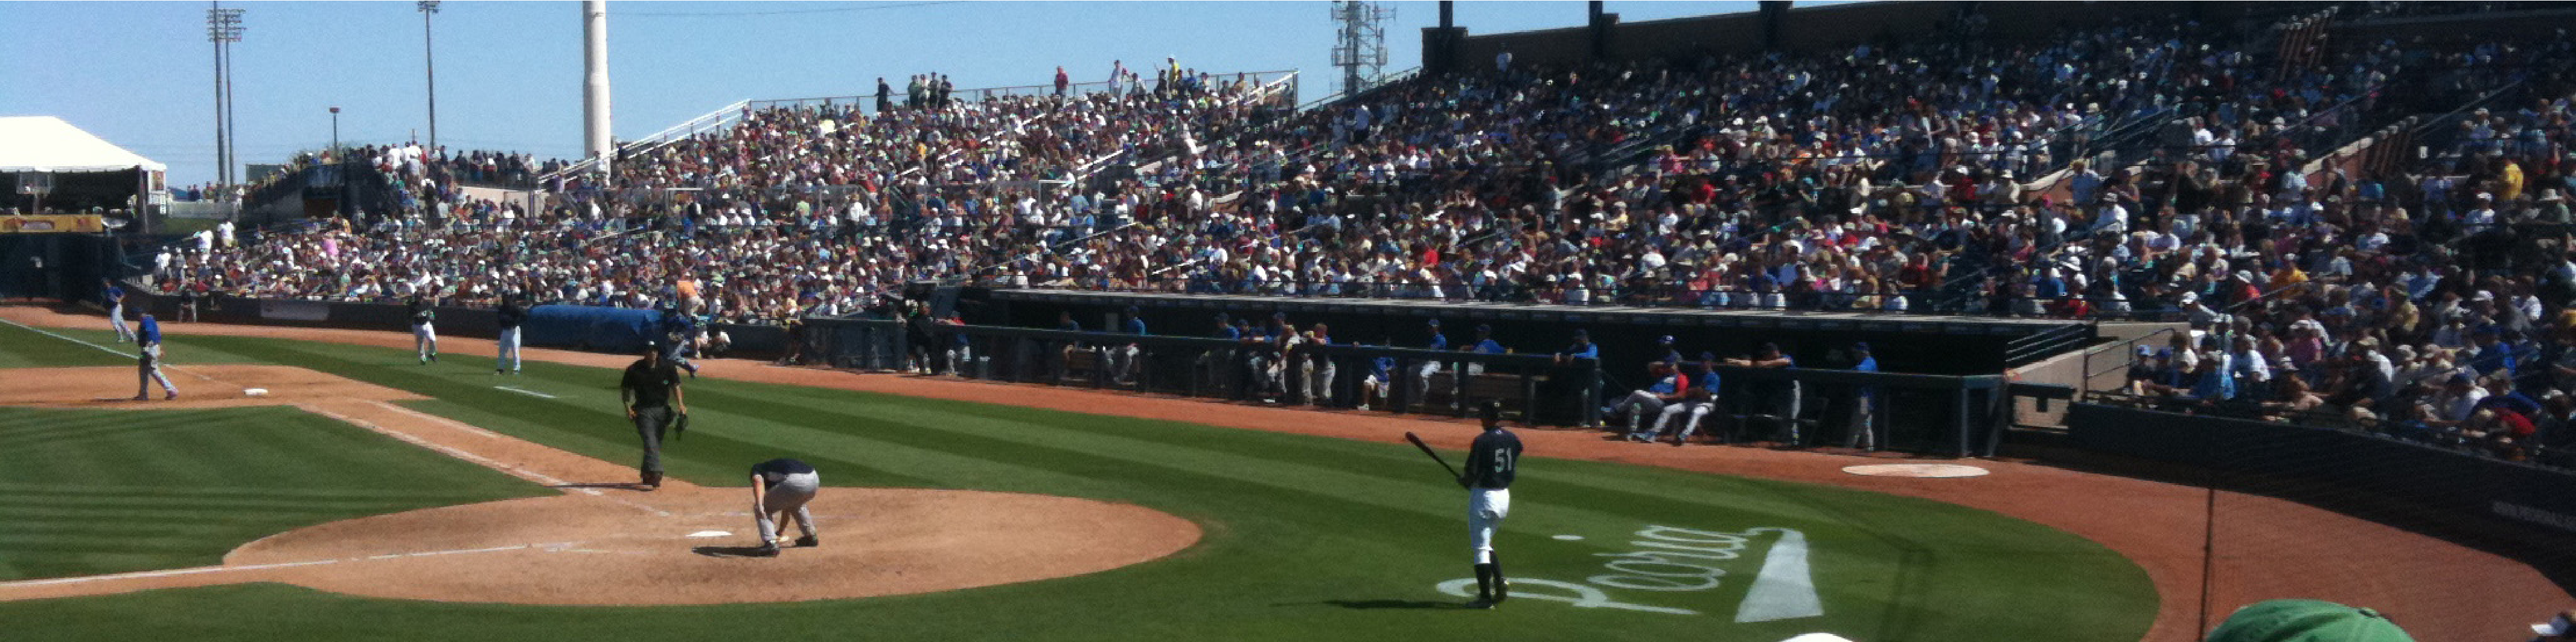
\includegraphics[width=\textwidth]{images/sampleteaser}
%   \caption{Seattle Mariners at Spring Training, 2010.}
%   \Description{Enjoying the baseball game from the third-base
%   seats. Ichiro Suzuki preparing to bat.}
%   \label{fig:teaser}
% \end{teaserfigure}

%%
%% This command processes the author and affiliation and title
%% information and builds the first part of the formatted document.
\maketitle
